\documentclass{sig-alternate}
%\usepackage{times}
\usepackage{url}
\usepackage{epsfig}
\usepackage{footnote}
\usepackage{amsmath}
\usepackage[small,it]{caption}

%\hyphenpenalty=10000
%\tolerance=10000

\setlength{\parskip}{0pt}
\setlength{\parsep}{0pt}
\setlength{\headsep}{0pt}
\setlength{\topskip}{0pt}
\setlength{\topmargin}{0pt}
\setlength{\topsep}{0pt}
\setlength{\partopsep}{0pt}
\setlength{\floatsep}{5pt}
\setlength{\textfloatsep}{5pt}
\setlength{\intextsep}{5pt}

\begin{document}


\twocolumn[%
\centerline{\Large \bf OverSoc: Social Profile Based Overlays} 
  \medskip
  \centerline{\bf David Isaac Wolinsky, Pierre St. Juste, P. Oscar Boykin, Renato Figueiredo}
  \centerline{\bf University of Florida}
  \bigskip
]

%\title{OverSoc: Social Profile Based Overlays}

%\numberofauthors{1}

%\author{
%\alignauthor
%David Isaac Wolinsky,
%Pierre St. Juste,
%P. Oscar Boykin,
%Renato Figueiredo \\
%\affaddr{University of Florida}
%}

%\maketitle

\begin{abstract}

Online social networking has quickly become one of the most common Internet
activities.  As social networks evolve, they encourage users to share more
information, requiring the users, in turn, to place more trust into social
networks.  In centralized systems, this means trusting a third-party commercial
entity, like Facebook or MySpace.  Peer-to-peer (P2P) systems can enable the
creation of online social networks extending trust to friends only.  In this
paper, we present a novel approach to constructing completely decentralized
social networks through P2P overlays, OverSoc.  Our approach relies on a common
directory overlay, which facilitates friend discovery and bootstraps
connectivity to individualized profile overlays.  Each user has their own
individual profile overlay managed transparently using a public key
infrastructure (PKI).  We define necessary interfaces for constructing the
system and describe some examples of user interactions with the system.

\end{abstract}

\section{Introduction}

Online social networking has become pervasive in daily life, though as social
networks grow so does the wealth of personal information that they store.
Once information has been released on a social network, known as a user's
profile, the user and the data are at the mercy of the terms dictated by the
social network infrastructure, which today is typically third-party, centrally
owned.  If the social network engages in activities disagreeable to the user,
due to change of terms or opt-out programs not well understood by users such
as recent issues with Facebook's Beacon program~\cite{facebook_beacon}, the
options presented to the user are limited.  The options include leaving the
social network, surrendering their identity and features provided by the social
network; accepting the disagreeable activities; or to petition and hope that
the social network changes its behavior. 

As the use of social networking expands to become the primary way in which
users communicate and express their identity amongst their peers, the users
become more dependent on the policies of social network infrastructure owners.
Recent work~\cite{p2p_socialnetwork} explores the coupling between social
networks and P2P systems as a means to return ownership to the users, noting
that a social network made up of social links is inherently a P2P system with
the aside that they are currently developed on top of centralized systems.  In
this paper, we extend this idea with focus on the topic of topology; that is,
how to organize social profiles that leverage the benefits offered by a
structured P2P overlay abstraction.

Structured P2P overlays provide a scalable, resilient, autonomic platform for
distributed applications.  Structured overlays enable users to easily create
their own decentralized systems for the purpose of data sharing, interactive
activities, and other networking-enabled activities.  In this paper, we extend
our previous work~\cite{vpo} to enable social network profile overlays.  The
previous work addresses the challenges of bootstrapping secure, private
overlays in NAT and firewall environments by using a public overlay for
discovery and as a relay or communication transport.  

A typical social network consists of users and groups.  Each user has a
profile, a set of friends, and private messaging; and each group consists of
one or more managers, users, and a messaging board.  Profiles contain user's
personal information, status updates, and public conversations, similar to a
message board.  Friends are individuals trusted sufficiently by a user to view
the user's profile.  Private messaging sends messages discretely between users
without leaking the message to other members.  Groups have similar features,
though identity is shared by many users.

Using this social networking model, we have designed OverSoc.  OverSoc uses a
public overlay can be used as a directory for finding and befriending peers or
finding and accessing groups.  Once group and profile access has been offered,
the public overlay can be used to bootstrap connectivity to existing profile
and group overlays.  Security for profile are provided by a public key
infrastructure (PKI), where profile owners or group managers are the
certificate authorities (CA) and all members have signed certificates.  The
overlay stores profile data or group information in its distributed data store,
supporting decentralized access using scalable mechanisms regardless of the
profile owner's online presence.  In this paper, we present the architecture of
these overlays, as presented in Figure~\ref{fig:system}.

\begin{figure}[h]
\centering
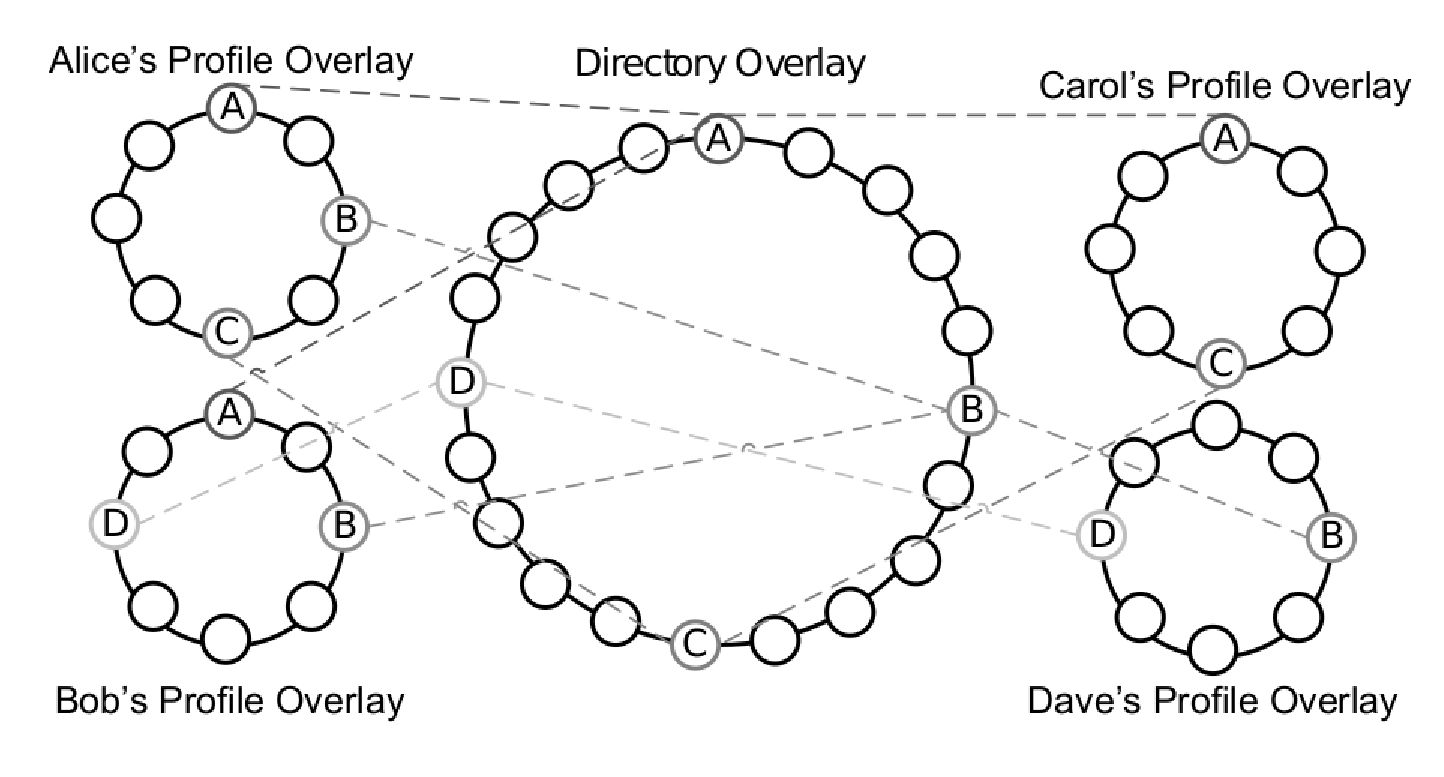
\epsfig{file=figs/subrings.eps, width=3.12in}
\caption{An example OverSoc social overlay network.  Alice has a friendship
with Bob and Carol, hence both are members of her profile overlay. Bob has a
friendship with Alice and Dave but not Carol; hence Alice and Dave are members
of his profile overlay, while Carol is not.  Each peer has many overlay
memberships but a single root represented by dashed lines in various shades of
gray.  For clarity, overlay shortcut connections are not shown.}
\label{fig:system}
\end{figure}

The rest of this paper is organized as follows.  Section~\ref{background}
provides background and related work.  Section~\ref{social_overlays} describes
OverSoc, explaining how to map social networks onto structured P2P overlays.
We express our expectations for user interaction with the system in
Section~\ref{user_interaction}.  In Section~\ref{outstanding}, we explore some
of the remaining challenges introduced by our approach.  We conclude the paper
in Section~\ref{conclusion}.

\section{Background}
\label{background}

In this section, we review structured P2P overlays, challenges and solutions
for bootstrapping overlays, and other methods for constructing decentralized
online social networks.  P2P systems build upon existing decentralized concepts
by creating scalable, autonomic environments, thereby limiting user exposure to
the gory details of system configuration and organization.  Since our system
consists of many profile overlays, we focus on the challenges of bootstrapping
P2P systems, when the system lacks dedicated bootstrapping nodes.

\subsection{Structured P2P Overlays}

P2P systems typically come in two flavors:  unstructured and structured.
Unstructured systems are generally constructed by peers attempting to maintain
a certain amount of connections to other peers in the P2P system, whereas
structured systems organize into well-defined topologies, such as 2-D rings or
hypercubes.  Though unstructured systems are typically simpler to bootstrap and
maintain, they rely on global knowledge, flooding, or stochastic techniques to
search for information in an overlay and thus creating potential scalability
constraints.  Alternatively, structured systems have guaranteed search time
typically with a lower bound of $O(\log N)$, though recent research has shown
that these systems can be constructed to support $O(1)$ search time.  Some
examples of structured systems are Pastry~\cite{pastry}, Chord~\cite{chord},
Symphony~\cite{symphony}, Kademlia~\cite{kademlia}, CAN~\cite{can}, and
Dynamo~\cite{dynamo}.

A key component of most structured overlays is support for decentralized
storage / retrieval of information by mapping keys to specific node IDs in an
overlay called a distributed hash table (DHT).  At a minimum, the data is
stored at the node ID either smaller or larger to the data's node ID and for
fault tolerance the data can be stored at other nodes.  DHTs can be used by
peers of systems to coordinate allocation and discovery of resources, making
them attractive for self-configuration in decentralized collaborative
environments.  DHTs provide the building blocks to form more complex
distributed data stores as presented in Past~\cite{past} and
Kosha~\cite{kosha}.

One of the key challenges to overlays is the bootstrapping problem, that is,
how does one find an active member in the overlay in order to become a member.
In large public systems, often times, the owners of the project and sometimes
corporate sponsors provide these resources, though these types of bootstrapping
peers are typically not available for small, private overlays.  The
bootstrapping problem can be divided into two components: finding a
bootstrapping member of the overlay and handling connectivity constraints if
the overlay has no members with public addresses.  In~\cite{one_ring,
can_multicast}, the authors discuss the concept of a single overlay supporting
services through the use of additional overlays, which use the underlying
overlay to assist in discovery, this deals with the component of finding a
bootstrap peer.  To address the challenge of bootstrapping peers behind NATs,
we described a system in~\cite{vpo}, which enables the public overlay to act as
a NAT traversal rendezvous point.  More specifically, a peer, attempting to
join a private overlay, queries the public overlay's DHT to obtain a list of
currently online private overlay peers who have matching public IDs.  The peers
then use the public overlay, in addition to direct UDP or TCP links, to
communicate with the private overlay nodes and bootstrap into the private
overlay.  This method enables peers even behind firewalls and NATs to have
publicly available addresses in the public overlay.  Additionally this work
describes mechanisms that enable the use of PKI technologies to seamlessly
secure both point-to-point and end-to-end communication in a structured
overlay.

\subsection{Peer-to-Peer Social Networks}

In~\cite{peerson}, Buchegger et al. describe how to use a DHT to store social
networking profile.  The DHT provides look-up services for storing meta data
pertaining to a peer's profile.  Peers query the DHT for updated content from
their friends by hashing their unique identifiers (e.g. friends' email
addresses).  The retrieved meta data contains information for obtaining the
profile data such as IP address and file version. Their work relies on a PKI
system that provides identification, encryption, and access control.  In
contrast, OverSoc users and groups have their own private overlay secured by
point-to-point encryption and authentication amongst all peers in the overlay.
The private overlay provides a clean abstraction of access control, whereby
once admitted to a private overlay, users can access a distributed data store
which holds the contents of the owners profile.

Shakimov et al. in \cite{vis-a-vis} take a different approach by depending on
virtual individual servers (VIS) hosted on a cloud infrastructure such as
Amazon EC2. Friends contact each other's VIS directly for updates.  A DHT is
used as a directory for groups and interest-based searches. Their approach
assumes bidirectional end-to-end connectivity between each VIS, where a profile
is only available during the up time of the VIS.  Because of the demands on
network connectivity and up time, the approach assumes a cloud-hosted VIS and
has difficulty being used on user-owned resources.  OverSoc allows peers to
have  asymmetric connectivity and does not require constant up time through the
use of NAT traversal support and the ability to store the profile in the
overlay's distributed data store.

The approach presented by Cutillo et al. in~\cite{matryoshka} relies on a
central system to host identities and certificates that can then be used to
query a DHT to discover an initial hop in a route to a specific peer through
their circle of friends.  The circle of friends consists of an unstructured
overlay, where direct friends maintain direct connections with the peer, and
outer circles consist of friends of friends and friends of friends of friends.
The main goal of this work is to remove the private components of a profile
from a central entity, whereas OverSoc makes a clean break from all
centralization and emphasizes scalability through distributed replica
techniques.

Unlike the above approaches, the P2P social network presented by Abbas et al.
in~\cite{tribler-osn} uses an unstructured overlay without a DHT where peers
connect directly to each other rather than through the overlay establishing
unique identifiers to deal with dynamic IPs.  Peers cache each other's data to
improve availability.  While helper nodes are used to assist with
communication between peers behind NATs.  The approach lacks security and
access control considerations and lacks the guarantees and the simplicity of
the abstraction offered by a structured overlay.

\section{Social Overlays}
\label{social_overlays}

In this section, we explain how OverSoc maps online social networking to
virtual private overlays consisting of a public directory overlay with many
private profile overlays.  The directory overlay supports friend discovery and
verification and stores a lists of peers currently active in each profile
overlay.  Profile overlays support message boards, private messages, and media
sharing.

\subsection{Finding Friends}

In a traditional social network, directories are used to search for users based
upon public information, such as the user's full name, user ID, e-mail address,
group affiliations, and friends.  The resulting search returns zero or more
matching directory entries.  In OverSoc, directory entries are inserted into
the DHT of a public overlay.  Since the public information has many components,
various subsets form DHT keys that all point to a common, complete listing of
the matching public information.  For example, a user can store a pointer at
the DHT key $hash("alice")$ or $hash("alice bob")$.  The key here is that any
subset of the user's public information in lower-case format can be hashed into
a DHT index that would eventually direct the searching user to one or more
users public information.  More explicit searches could sift through the
results and present to the user only those peers, which match all the search
parameters.  The amount of information shared publicly should be configurable
by the user.

While looking for an individual, a peer may discover that many individuals have
overlapping public information components, such as the user's name.  Assuming
all entries are legitimate, the overlay must have some method of supporting
multiple, distinct values at the same key, requiring the application and user
to parse the responses and determine the best match by reviewing the contents
of each certificate.  Alternatively, a technique like Sword~\cite{sword}, which
supports distributing the data across a set of nodes and using a bounded
broadcast to discover peers that match all information, could be used for
searching.

To address trust levels when searching for friends, a PGP certificate can be
used to store user's public information and verify user's friends and groups.
In OverSoc, the main portion of a PGP certificate contains information such as
user name, full name, e-mail address, potentially other user-defined data, and
a signature packets from the user and those that trust the certificate
including groups and individuals.  These signature packets represent a list of
verifiable friends and groups assisting to further uniquely identify a user.
Each time a user befriends someone, they should exchange signature packets
containing at a minimum the friends PGP certificate ID, a signature expiration
time, and a signature binding this information with the new friend's existing
PGP certificate.  This increases the trust level of individuals searching for
others especially if they have common friendships or group membership.  The use
of a time stamp in the signature assists in deciding whether or not a
friendship link is still active without accessing the profile overlay of either
peers.  Thus peers that maintain friendships need to periodically exchange
signature packets.

\subsection{Making Friends}

Once a user, \textit{Alice}, has found a friend candidate, \textit{Bob},
\textit{Alice} can issue a friendship request and store it in the DHT using the
hash of Bob's certificate as an index, this acts a public overlay mailbox.
\textit{Bob} can review the public information of \textit{Alice} prior to
making a decision.  If \textit{Bob} accepts the request, \textit{Alice} and
\textit{Bob} exchange signature packets and are granted access to each other's
profiles.  Once profile access has been enabled, the \textit{Alice} and
\textit{Bob} can learn more information, and if it turns out to be a mistake,
either one of them can unilaterally end the relationship.

Alice's friendship request should contain a pointer to her certificate in the
overlay, a time stamp, and Bob's certificate identifier.  The friendship
request is encrypted using Bob's public key and signed using Alice's private
key for the purposes of anonymity and authenticity.  When Bob receives the
friendship request, he can verify that the request was made for Bob by Alice.
Upon receiving the friendship request, he has three choices:  a conditional
accept, an unconditional accept, or a reject.  During an unconditional accept,
Bob signs Alice's PGP certificate and issues a request to befriend her.
Alternatively, he could issue a request to befriend her and wait for her to
sign his certificate and investigates her profile prior to signing hers.

Discovery of a user is not limited to the directory entries.  Because users
have a public overlay based mailbox, they are not required to discover each
other only through the directory.  Instead, they can use out of band discovery,
using mechanisms like e-mail, chat, or personal websites to exchange
certificates.  Once a peer has received another peer's certificate, they can
submit secure friendship requests using the public overlay.

\subsection{The Profile Overlay}
\label{profile_overlay}

In a traditional social network, the profile or user-centric portion consists
of private messaging, data sharing, friendship maintenance, and a public
message board for status updates or public messages.  In this section, we
explain how these components can be applied to a structured overlay dedicated
to an individual profile.

Using the techniques such as those described in~\cite{vpo}, it is feasible to
efficiently multiplex a P2P system across multiple, virtual private overlays
enabling each profile owner to have a profile overlay consisting of their
online friends.  For access control, OverSoc employs point-to-point encryption
and authentication, peers bootstrap private connections by exchanging the base
of the PGP certificate and the profile overlays signature packet obtained in
the ``making friends'' stage.  Because the profile owner also is the CA for all
members of the overlay, they can easily revoke users from access to the profile
overlay.  \cite{vpo} describes efficient mechanisms for overlay revocation
through the use of broadcasting for immediate revocation and the use of DHT for
indirect and permanent revocation.

The message board of a profile can be stored in two ways: distributed within
the profile overlay via a data store or stored on the profile owner's personal
computing devices.  The distributed data store provides the profile when the
owner is offline and also distributes the load for popular profiles.  For
higher availability, each peer always stores and provides all data in their
profile when they are online.  To ensure authenticity and integrity, peers sign
their messages and each peer's certificate is available in the overlay as well
as stored by mutual friends for verification.  Messages that are unsigned are
ignored by all members of the overlay.  An ideal overlay for this purpose
should support complex queries~\cite{complex_queries} allowing easy access to
data stored chronologically, by content, by type, i.e., media, status updates,
or message board discussions.

Private messaging in the profile overlay is unidirectional; only the profile
owner can receive private messages using their overlay.  To enforce this, a
private message should be prepended with a symmetric key encrypted by the
profile owners public key, the message should be appended by a signature of the
message using the private key of the message sender, and the entire message
encrypted by the symmetric key.  This approach ensures that only the sender and
the profile owner can decrypt the private message and verify the senders
identity.  The contents of the private message include the sender, time sent,
and the subject.  Messages are be stored in well known locations in the DHT,
like ``private messages for me'', so that the profile owner can either poll the
location.

%\subsection{Event Based Message Notification}

%Both the directory and profile overlays have methods by which peers can receive
%messages.  In the directory overlay, these take form by means of friendship
%requests and friendship accepts, certificate signature packets.  The profile
%overlay supports private messages.  While polling the location in the DHT
%occasionally will allow peers to receive the messages, polling has inherent
%delays and network costs.  Alternatively, event  enable peers to receive sent
%messages very quickly after they have been sent with minimal impact on network
%throughput.

%A simple method for implementing an event notification system involves using
%the DHT.  Each event would have an identification that would map to a list of
%peers wanting to know when an event occurred and the data associated with it.
%Thus mapping the $(event id, listener)$ to the DHT could be done by hashing a
%string such as ``private messages for me'' or taking a hash of the user's
%certificate hash for public overlay messages and storing the profile owners
%active nodes into the list of listeners .  When a message is inserted into the
%user's mailbox, the sender could query this list and send to each listener a
%notification of the new private message.  Alternatively, if a higher degree of
%anonymity is required, the DHT server could be modified to forward the response
%to the listeners directly rather than returning a list of listeners.  Of
%course, this does not prevent potential race conditions occurring, such as a
%situation where a peer recently joined their profile overlay, had already
%queried their mailbox and found it empty, while simultaneously a private
%message was sent to them yet they were not in the listeners list.  Thus
%occasional polling is required, though can be minimized, the longer a node has
%been online.

\subsection{Active Peers}

The directory overlay should be used to assist in finding currently active
peers in the profile overlays.  By placing their node IDs at a well-known,
unique per-profile overlay keys in the DHT, active peers can bootstrap
incoming peers into the profile overlay.  We implemented and evaluated this
concept in~\cite{vpo}.  Because the profile overlay members all use PKI to
ensure membership, even if malicious peers insert their ID into the active
list, it would be useless as the peer would only form connections with peers
who also have a signed certificate.

\subsection{Groups}

Groups can be considered extensions of profile overlays.  The fundamental
difference between a group and a profile is that a group lacks private
messaging and has shared ownership.  So just as a peer can find a profile in
the directory by hashing the name of the user and other identifiable
information, so can the user find the group.  Like the certificate of the user,
the members of a group sign the group's certificate to represent their
membership to that group.  In OverSoc, users request membership to the group
like they do friendship requests, in response a group manager can sign their
certificate allowing that member access to the group.  Finally, the group can
be bootstrapped in the same way as the profile overlay through the directory
overlay.

The unique challenge presented by groups is the sharing of the CA task.  A
decentralized solution would be for all members of the group to be listed in
the groups DHT and when a peer becomes a manager, they obtain a new signature
packet that contains a user-defined component stating that they are managers.
If an administrator loses their position, then all members who had their
certificate signed by that administrator would need to obtain a new
certificate.  To avoid member churn, the owner could provide signature packets
for all group members.  Thus the managers just allow temporary access until the
owner comes online and provides more permanent access.

\section{User Interaction}
\label{user_interaction}

OverSoc consists of many components that are transparent to the user, the user
experience should appear to the user no differently than an existing online
social network.  The OverSoc could be a downloadable application or a browser
based Flash or Silverlight application.  If the user, Bob, had already created
an account, Bob would be presented with an interface showing their friends
profiles.  Based upon Bob's configuration, the social application could
retrieve profile updates as he navigates to individual profiles or as soon as
the application joins an individual profile overlay, reactive versus proactive
profile querying.  

If this was Bob's first time starting OverSoc, he would be presented with
screens asking for his privacy preferences, such as whether or not he wants his
information in the directory overlay, if he felt comfortable enough with the
idea of people knowing he was a member of the social network and who his
friends are.  Then OverSoc would ask for personal information to populate his
profile and to generate his directory information.  At which point, the OverSoc
would join the overlay and create Bob's private overlay.  Bob could then start
searching for friends, make friend requests, and respond to friend requests.

Recently, Bob had been thinking about his high school days and was curious if
Alice was also a member of OverSoc, though Bob did not have Alice's e-mail
address, just her first and last name.  Bob enters Alice's name into the
OverSoc search box and is presented by a list of Alice's.  As Bob reviews each
of the entries, he recognizes an Alice that is friend's with some of the same
people Bob was in high school.  Bob selects to become her friend.  At which
point, the OverSoc transparently inserts a friendship request to Alice and
signs Alice's certificate so Alice can view Bob's profile.  Of course that is
because Bob has chosen to allow user-initiated friend requests access to his
profile.  Alice receives Bob's request, peruses his profile and feels fine
becoming friends with Bob, which initiates a transparent process of signing
Bob's certificate and placing the result in the public overlay.  There is one
problem though, when Bob receives Alice's signature and views her profile, he
realizes that this is some other Alice.  He quickly chooses to defriend her.
This causes Bob's OverSoc instance to broadcast a revocation for Alice's
signature and to store the revocation in the DHT.  Alice, who was viewing Bob's
profile, is notified of this sudden loss of trust and while she is able to view
the contents of Bob's profile, which she has already accessed and obtained, she
can no longer receive updates as members of Bob's overlay prevent her from
accessing it.

%In another instance, Bob bumped into Carol, who e-mailed Bob a copy of her
%certificate.  Bob points OverSoc to the certificate, and OverSoc verifies that
%he wants to become friends with the identity associated with the certificate.
%When he accepts, OverSoc immediately submits a request to become Carol's
%friend.  Carol receives notification and accepts Bob's friendship request.  At
%this point, both Bob and Carol have transparently exchanged signed certificates
%and have mutual access to each other profiles.  As Bob reads Carol's latest
%news, he remembers a funny personal story and that he would like to share with
%Carol.  So he sends Carol a private message.  Carol is offline though.  The
%next time Carol goes online, her social application discovers the message and
%presents it to her.  In this scenario, OverSoc  has taken the private message,
%secured it with her public key and a symmetric key and signed it with his
%private key.  After which, it inserts the message into the DHT and sends a
%notice to the event notification system, which detects that there were no
%listeners.  When Carol's application comes online, it queries the DHT receiving
%the message.  Prior to presenting Carol the message, the OverSoc decrypts and
%verifies the message.

\section{Challenges}
\label{outstanding}

While structured P2P overlays have been well-studied in a variety of
applications, their use in social profile overlays raises new interesting
questions, including:

{\bf 1) Handling small overlay networks} - P2P overlay research typically
focuses on networks larger than the typical user's friend count (Facebook's
average is 130\footnote{http://www.facebook.com/press/info.php?statistics}).
Because social profile overlays are comparatively smaller, this can impact the
reliability of the overlay and availability of profile data.  A user can host
their own profile; however when the user is disconnected it is important that
their profile remains available even under churn. It is thus important to
characterize churn in this application to understand how to best approach this
problem. An optional of per-user deployment of a virtual individual server
(VIS) and the use of replication schemes aware of a user's resources provide
possible directions to address this issue.

{\bf 2) Overlay support for low throughput, unconnected devices} - devices such
as smart phones cannot constantly be actively connected to the overlay and the
connection time necessary to retrieve something like a phone number may be too
much to make this approach useful.  Similar to the previous challenge, this
approach could benefit from using a VIS enabling users access to their social
overlays by proxy without establishing a direct connection to the overlay
network.

{\bf 3) Reliability of the directory and profile overlay} - Overlays are
susceptible to attacks that can nullify their usefulness.  While the profile
overlay does have point-to-point security, in the public, directory overlay,
the lack of any form centralization makes policing the system a complicated
procedure.  While our approach of appending friends list can assist users in
making decisions on identity, it does not protect against denial of service
attacks.  For example, users could attempt create many similar identities in
an attempt to overwhelm a user in their attempt to find a specific peer.
Previous work has proposed methods to ensure the usability of overlays even
while under attack.  For the social overlay to be successful, we must identify
which methods should be used. A possible approach is to replicate public
information within a user's profile overlay thus providing an alternative
directory overlay for querying prior to using the public directory overlay.

\section{Initial Results}
\label{experiments}

This environment presents many challenges in terms of providing user seamless
similar to that of a centralized environment.  Using tools that we developed
to evaluate the virtual private overlays, we performed some experiments that
focus on connectivity times to profile overlays and querying data in the
directory overlay.  Both systems were evaluated using a network modeling tool,
though the virtual private overlay technique was also tested using PlanetLab
using Brunet~\cite{brunet}, a P2P framework supporting virtual private overlays.

To evaluate the public overlay, peers first queried the DHT to obtain a pointer
to a certificate and then obtained the certificate in a following request.  So
the result presented is effectively the time it takes to make two requests into
a DHT.  Using the network modeling tool, the average time for a network size of
100,000 was 4.04 seconds.

To evaluate the virtual private overlays, we created various sized public and
private overlays and determined the time it took for a new peer to join both
overlays.  The incoming peer joined the public overlay, then queried the public
DHT for members active in the private overlay.  At which point, the peer
created another private overlay node and used these results to bootstrap
connections into the private overlay.  When the private overlay node became
connected, the correct peer on both sides, as determined by the structured
overlay, the test was completed.  In the PlanetLab experiments, the public
overlay consisted of 600 nodes and a random distribution of peers in the
private overlay with point-to-point security links enabled, the time to connect
was less than 22 seconds.  The network modeler focused on larger systems, up to
100,000 peers in both overlays.  In these environments, it never took longer
than 48 seconds to become connected to both overlays.

\section{Conclusion}
\label{conclusion}

In this paper, we proposed OverSoc, a system that constructs a decentralized
online social network through the use of structure P2P overlays.  P2P systems,
in general, have very nice properties that make them attractive for average
users.  Namely, they require minimal configuration and organization of
resources, in addition, P2P systems naturally handle increased demand due to
additional peers.  Our approach is based upon the use of a multiple overlay
system, where all users join a public directory overlay which assists in
finding friends and groups and bootstrapping into their private overlays.  When
making a friendship or joining groups, peers exchange signatures that enable
access to each others overlays.  Each private overlay employs point-to-point
encryption and authentication so that only trusted peers can access the
overlays.  The use of unique overlays for each profile and group allows a clean
abstraction for privacy purposes that simplifies security handling of access to
private data.  Existing work in the realm of structured overlays describes
mechanisms for efficiently and securely storing profile information into the
profile overlay.  Our proposed system returns control of the social network and
more importantly users' identity to the users and eliminates the need for
centralized social networks.\\

{\small
\bibliographystyle{abbrv}
\bibliography{SocialProfileOverlays}
}

\end{document}
